%!TEX root = ../IfN-LaTex.tex
%!TEX spellcheck

\chapter{Evaluation}
\label{chap:Evaluation}

In this chapter the developed broadband and sub-band post-processing algorithms are evaluated and compared to the algorithm proposed by Madhu. To realize this they were implemented with \emph{Matlab}. The evaluation process is shown in figure \ref{fig:overview_eval}. The Input signals for the \ac{ASL} are the microphone signals $x(n)$ from a 7 microphone \ac{UCA+C} which has a radius of \SI{42}{\milli \metre}. The microphone signals are transformed by the \ac{STFT} to obtain the signals $\vect X(l,b)$ in time-frequency representation. The \ac{ASL} (described in chapter~\ref{sec:alg_localization}) acquires the signals and processes them by steering the \ac{DS} or Capon beamformer within a search grid of directions. The steered power spectrum is obtained and passed to the maximum search, based on the \ac{SRP} for broadband or in every sub-band. The raw localization is used to calculate the confidences (Chapter~\ref{sec:confidence}). Confidences and \ac{SRP} localization results are then directed to the different kinds of post-processing algorithms. For comparison the Madhu algorithm was implemented. Finally, classification results are directed to the evaluation where different metrics are calculated.\\

This chapter begins with discussing the modification of Madhu's post-processing algorithm, which is used as a reference. Then the evaluation setup is stated and the system setup is described, showing the parameter tuning for the different algorithms. The dataset of microphone signals is separated into a development set for tuning and a test set, where the final evaluation is conducted.\footnote{This is done to achieve independent results and avoiding results that are overfitted on the development set.} In the following section the results of all algorithms are stated and discussed afterwards. Finally, the results are wrapped up and a conclusion is drawn.



\begin{figure}[!ht]
	\centering
    % \def\svgwidth{1\linewidth}
    % Author: Rasmus Pank Roulund

\usetikzlibrary{calc,trees,positioning,arrows,chains,shapes.geometric,%
    decorations.pathreplacing,decorations.pathmorphing,shapes,%
    matrix,shapes.symbols,fit}

\tikzset{
>=stealth',
  rect/.style={
    rectangle,
    rounded corners,
    % fill=black!10,
    draw=black, very thick,
    text width=8em,
    minimum height=3em,
    text centered
    },
  group/.style={
    rectangle,
    rounded corners,
    % fill=black!10,
    draw=black, dashed, thick,
    text width=8em,
    minimum height=3em,
    text centered
    },
  line/.style={draw, thick, ->},
  line2/.style={draw, thick, -},
  element/.style={
    tape,
    top color=white,
    bottom color=blue!50!black!60!,
    minimum width=8em,
    draw=blue!40!black!90, very thick,
    text width=10em,
    minimum height=5em,
    text centered,
    on chain},
  every join/.style={->, thick,shorten >=1pt},
  decoration={brace},
  tuborg/.style={decorate},
  tubnode/.style={midway, right=2pt},
  coordinate/.style={minimum height=3em,},
}

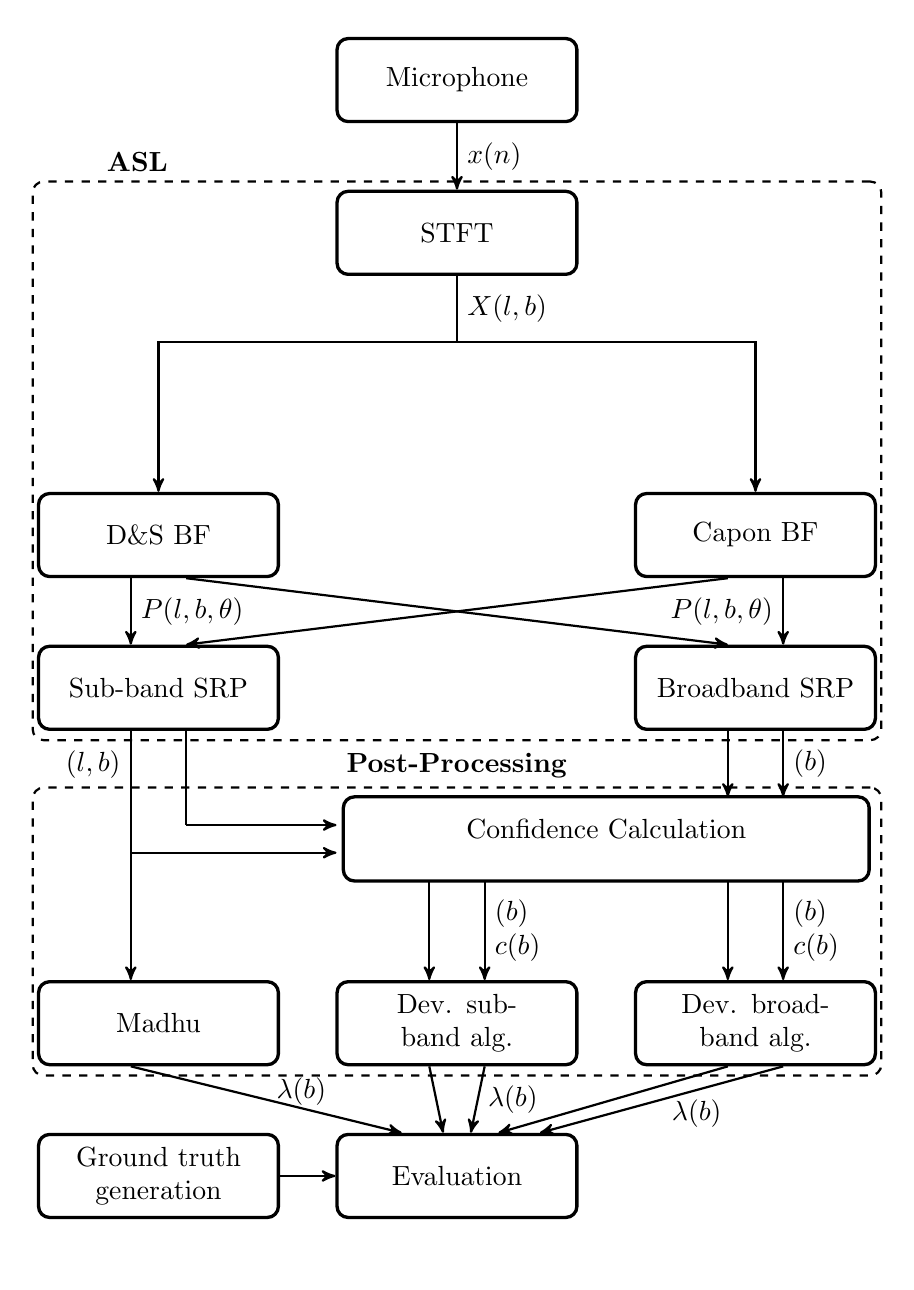
\begin{tikzpicture}


	\matrix (m1) [row sep=1.2em, column sep=2em]
	{
		\node[coordinate] 	(m01) {};          		&
		\node[rect]       	(m02) {Microphone};     	&
		\node[coordinate] 	(m03) {};          		\\
	\\
		\node[coordinate] 	(m11) {};          		&
		\node[rect]       	(m12) {STFT};		     	&
		\node[coordinate] 	(m13) {};          		\\
	\\
		\node[coordinate] 	(m21) {};          		&
		\node[coordinate]	(m22) {};		     	&
		\node[coordinate] 	(m23) {};          		\\
	\\
		\node[rect] 		(m31) {D\&S BF};     		&
		\node[coordinate]   (m32) {};		     	&
		\node[rect] 		(m33) {Capon BF};    		\\
	\\
		\node[rect] 		(m41) {Sub-band SRP};     		&
		\node[coordinate]   (m42) {};		     	&
		\node[rect] 		(m43) {Broadband SRP};    		\\
	\\

		\node[coordinate] 	(m51) {};          		&
		\node[coordinate, minimum height=3em,]	(m52) {};		     	&
		\node[coordinate] 	(m53) {};				\\
	\\
		% \node[coordinate] 	(m61) {};          		&
		% % \node[coordinate, minimum height=3em]	(m62) {};		     	&
		% \node[coordinate] 	(m63) {};				\\
	\\
		\node[rect] 		(m71) {Madhu};     		&
		\node[rect]		   	(m72) {Dev. sub-band alg.};		     	&
		\node[rect] 		(m73) {Dev. broadband  alg.};    		\\
	\\
		\node[rect]	(m81) {Ground truth generation};     		&
		\node[rect]		   	(m82) {Evaluation};		     	&
		\node[coordinate]	(m83) {};    		\\
	\\
	};
	\node[rect, inner sep=0pt ] (outer) [fit=(m52) (m53),text width=19em] {Confidence Calculation};
	\node[group, outer sep=0em, label=above left:{\textbf{ASL}} ] (outer) [fit=(m11) (m13) (m41) (m43),text width=30em] {};
	\node[group, outer sep=0em, label=above:{\textbf{Post-Processing}} ] (outer) [fit=(m51) (m53) (m71) (m73),text width=30em] {};

	\draw[line] (m02) -- node [right]  {$x(n)$} (m12);
	\draw[line2] (m12) -- node [right]  {$X(l,b)$} (m22);
	\draw[line] (m22.north) -| (m31.north);
	\draw[line] (m22.north) -| (m33.north);
	\draw[line] ([xshift=-1em]m31.south) -- node [right]  {$P(l,b,\theta)$} ([xshift=-1em]m41.north);
	\draw[line] ([xshift=1em]m31.south) -- ([xshift=-1em]m43.north);
	\draw[line] ([xshift=1em]m33.south) -- node [left]  {$P(l,b,\theta)$}([xshift=1em]m43.north);
	\draw[line] ([xshift=-1em]m33.south) --  ([xshift=1em]m41.north);
	\draw[line] ([xshift=-0.6em, yshift=-0.5em]m51.west) --  ([xshift=-4em, yshift=-0.5em]m52.west);
	\draw[line2] ([xshift=1em]m41.south) -- ([xshift=1em, yshift=0.5em]m51.center);
	\draw[line] ([xshift=1em, yshift=0.5em]m51.center) -- ([xshift=-4em, yshift=0.5em]m52.west);
	\draw[line] ([xshift=-1em]m43.south) -- ([xshift=-1em]m53.north);
	\draw[line] ([xshift=1em]m43.south) -- node [right]  {$\phih(b)$}([xshift=1em]m53.north);
	\draw[line] ([xshift=-1em]m41.south) -- node [left, yshift=3.3em]  {$\phih(l,b)$} ([xshift=-1em]m71.north);
	\draw[line] ([xshift=-1em]m52.south) -- ([xshift=-1em]m72.north);
	\draw[line] ([xshift=1em]m52.south) -- node [right, yshift=0.6em]  {$\phih(b)$} node [right, yshift=-0.6em]  {$c(b)$} ([xshift=1em]m72.north);
	\draw[line] ([xshift=-1em]m53.south) -- ([xshift=-1em]m73.north);
	\draw[line] ([xshift=1em]m53.south) -- node [right, yshift=0.6em]  {$\phih(b)$} node [right, yshift=-0.6em]  {$c(b)$} ([xshift=1em]m73.north);
	\draw[line]([xshift=-1em]m71.south) -- node [right, yshift=0.3em]  {$\lambda(b)$}([xshift=-2em]m82.north);
	\draw[line]([xshift=-1em]m72.south) -- ([xshift=-.5em]m82.north);
	\draw[line]([xshift=1em]m72.south) -- node [right]  {$\lambda(b)$}([xshift=0.5em]m82.north);
	\draw[line]([xshift=-1em]m73.south) -- ([xshift=1.5em]m82.north);
	\draw[line]([xshift=1em]m73.south) --  node [right, yshift=-0.5em]  {$\lambda(b)$}([xshift=3em]m82.north);
	\draw[line](m81.east) -- (m82.west);
  \end{tikzpicture}

	\caption{Evaluation overview. First the different raw localization results $\phih$ are calculated by the acoustic source localization. Then multi-source classification algorithms calculate the classification results represented by the \acl{GMM} $\lambda$. For the evaluation the results of each algorithm are compared to the ground truth with different metrics.}
	\label{fig:overview_eval}
\end{figure}

\section{Reference Algorithm}
\label{sec:comp_alg}
As a reference the algorithm proposed by Madhu, as described in chapter \ref{subsec:madhu_alg}, is used. It should be noted, that it was developed to work with \ac{ULA} arrays and therefore has to be expanded for circular arrays. The classical \ac{EM}-algorithm is substituted with the one in chapter \ref{subsec:EM_for_WGMM} which is adapted for wrapped Gaussians. Furthermore the noise floor class is changed to a uniform distribution as stated in chapter \ref{subsec:floor}. A new threshold on the mixing coefficients is introduced $\Gamma_\text{affil}$ which is used to have a lower threshold for affiliations of observations to a class. This is added to the shrinking method:
if $\exists i$, such that $\pi_i < \Gamma_\text{affil}$
\begin{equation}
\begin{split}
\vect \mu &\leftarrow \vect \mu\  \backslash\ \mu_i \\
\vect \sigma^2 &\leftarrow \vect \sigma^2\ \backslash\ \sigma^2_i \\
\vect \pi &\leftarrow \vect \pi\ \backslash\ \pi_i \\
K &\leftarrow K-1.
\end{split}
\end{equation}
The backslash $\backslash$ means the set difference. In case the mixing coefficient constraint \ref{eq:pi_constraint} is violated, this is fixed with a reestimation of the parameter. The idea of using  a threshold for the mixing coefficient is mentioned in \cite{madhu2008scalable}, but is not integrated in his original implementation. However he used aliasing-free arrays and therefore did not have to deal with large amounts of 'false' detections. Therefore, the idea was implemented in the present work too. Last, the handling of overlapping sources, introduced in \ref{subsec:overlap} is also applied to the Madhu algorithm, to ensure a fair comparison.

%%- Adaption for Circular Arrays
\section{Evaluation Setup}
\label{sec:eval_setup}

In this section the evaluation setup is stated. First the microphone signal generation is presented. Then the \ac{GT} generation is introduced which is used to compare classification results within the evaluation. Finally the different evaluation metrics are explained.

\subsection{Microphone Signal Recordings}
\label{subsec:mic_rec_setup}
Microphone data were generated in an approximately 3m x 4m room with the \ac{UCA+C} array placed in the center of the room on a stand in about \SI{1.3}{\metre} of height (see figure \ref{fig:mic_rec_setup}). Omnidirectional \ac{MEMS} microphones were used together with phantom power supply. The microphones were installed upon a laser cut wooden plate depicted in figure \ref{fig:mic_array}. The signals are relayed to a soundcard which converts them to digitals for USB-transmission to a computer, where they are finally recorded. Data acquisition was conducted during different scenarios, i.e. with multiple human speakers and speaker boxes as sound sources. Speakers could be at one static position or roaming freely in the room. Their ways were crossing and during that they were speaking with interruptions. Distances of the speaker varied from $\SI{1}{\m}$ to $\SI{2}{\m}$. The full list of signal scenarios for development and test set can be viewed in the appendix \ref{tab:list_scenario}.

\subsection{Metrics}
\label{subsec:metrics}
To compare the developed post-processing algorithms, a broad set of metrics has to be evaluated. As a role model for the evaluation measures the field of visual object tracking is chosen. Here, a large variety of metrics exist, what can be inhibiting for the cross-paper comparison. To tackle this problem comprehensive review papers were written comparing and summarizing a broad field of measures \cite{yin2007performance,baumann2008review,vcehovin2016visual}. In that work the focus is on metrics for object classification but also on measures for accuracy. Because these measures are made for visual object tracking some of them had to be adapted for the developed acoustic multi-source algorithms. All measures are dependent on \ac{GT} tracks (Chapter~\ref{subsec:GT}), which are compared against the so called \ac{ST} tracks of the post-processing algorithm. An \ac{ST} track is defined as the mean value $\mu_k(b)$ of a class $k$ dependent on the frame index $b$.\\
Before the evaluation metrics are introduced concepts for temporal and spatial overlap have to be defined, which are used later by the different metrics. The temporal overlap is calculated for every GT-\ac{ST} pair. This is the number of frames where both tracks are present.
% , which can be stated as
% \begin{equation}
% TO_{sk}= \sum_{b = 1}^B \big(GT_s(b) \wedge ST_k(b)\big),
% \end{equation}
% where $GT_g(b)$ and $ST_s(b)$ are binary variables that state if a \ac{GT} track of source $s$ or \ac{ST} track of class $k$ is present in the frame $b$. They are compared by the binary \emph{AND} operator $\wedge$.
Spatial overlap is measured by the distance of a \ac{ST} track to the \ac{GT} track. If this distance is smaller than a threshold,
% $\Gamma_\text{SO}$
overlap is present in the frame $b$.
% , which can be written as
% \begin{equation}
% SO_{sk}(b) =
% \begin{cases}
% 1 & \text{for } |\varphi_s(b)-\mu_k(b)|<\Gamma_\text{SO}\\
% 0 & \text{for } |\varphi_s(b)-\mu_k(b)|>\Gamma_\text{SO}
% \end{cases},
% \end{equation}
% where $SO_{sk}(b)$ is the binary variable for spatial overlap, $\varphi_s(b)$ is the \ac{DOA} for source $s$, which is noted as the spatial location of our \ac{GT} track in frame $b$.
The mean $\mu_k(b)$ of class $k$ is taken as the \ac{ST} track's spatial location. The \ac{GT} generation is explained in a later chapter. In this work the spatial overlap threshold is set to
$\ang{35}$. As a more strict constraint for spatial overlap is the single source spatial overlap. Here the binary variable is only equal to one, when the \ac{ST} is the only one with spatial overlap.
% \begin{equation}
% SSO_{sk}(b) =
% \begin{cases}
% 1 & \text{for } |\varphi_s(b)-\mu_k(b)|<\Gamma_\text{SO}\ \wedge\ \sum_{k=0}^K\big(|\varphi_s(b)-\mu_k(b)|<\Gamma_\text{SO}\big) = 1\\
% 0 & \text{else}
% \end{cases},
% \end{equation}
With this stated the following metrics can be introduced.

\subsubsection{True Positives}
The \ac{TP} metric is actually a measure that is not considered in the final evaluation, but some of the following metrics are building on it. True positive is a \ac{ST} track when a \ac{GT} track can be assigned to it. This is done
by evaluation of a temporal overlap and a spatial overlap for a pair of \ac{GT} and ST. The constraint was adapted to be stricter by taking only the single source spatial overlap instead, in order to reduce double \acp{TP} for the same time span.
% \cite{yin2007performance}

\subsubsection{False Positives Duration}
All \ac{ST} tracks that have no \ac{TP} affiliation to any \ac{GT} track are considered as false positive. To have a more precise measure, in this work the false positive duration is considered as sum of the existence times of all false positives.
% Multiple \acp{TP} in the same time span were only added once.
By adopting this measure, the existence of long false positives can also be harmful in comparison to many short false positives. In the best case scenario the false positive duration would be zero.

\subsubsection{Root Mean Square Error}
The \ac{RMSE} is calculated for every \ac{TP} \ac{ST} track and when having spatial overlap. Spatial overlap is set as a condition because this should prevent \ac{ST} tracks that are totally drifting away from being considered and thus increasing the RMSE heavily.
% Therefore this part of the \ac{ST} tracks is also not taken into account for the track completion discussed in one of the next sections.
RMSE is a measure for the accuracy of the localization and should be zero in an optimal case.

\subsubsection{Track Interruptions}
Track interruptions indicate the lack of continuous tracking of a \ac{GT} track. When multiple \ac{ST} tracks are assigned to one \ac{GT} this is counted as interruption. Assigned is defined by the \ac{TP} measure. In optimal condition the track interruption should be zero.

\subsubsection{ID Change}

The metric \ac{IDC} is introduced for distinguishing if a \ac{ST} track is assigned to multiple \ac{GT} tracks. This can be seen as a mix-up of the classification. For this the single source spatial overlap is taken. If one \ac{ST} is assigned by single source spatial overlap to one source and after a time it is assigned to another source, then an \ac{IDC} happens. An example can be found in figure \ref{fig:results_idc}.

\subsubsection{Initial Detection Lag}
The initial detection lag measures the time gap between the start of the \ac{GT} track and the start of the first \ac{TP} \ac{ST} track. This indicates how fast the algorithm can detect new source appearances, which is an important measure when the localizer is used for wake up word detection in a speech recognition device. Overall the optimal latency should be zero.
% Large detection lags may mean that the system is not sensitive enough. Nevertheless, high sensitivity can evoke the FP count to rise.

\subsubsection{Track Completeness}
This metric measures the time overlap of \ac{GT} tracks and \ac{ST} tracks that is assigned as \ac{TP} to the \ac{GT} track, divided by the total time span of the \ac{ST} track. Multiple temporal overlap of multiple \ac{ST} tracks are only considered once. The measure is adapted in the way, that the \ac{ST} track must also have spatial overlap with the \ac{GT} track. Optimal track completion would be at $100\%$.

\subsubsection{Active Track Completeness}
Similarly to the track completeness the \emph{active} track completeness only allows for values of \ac{ST} tracks that are active. Activity is defined over the same threshold as the increase/decrease decision of the \ac{TTL} (equation \ref{eq:ttl_add}). This will give a measure for the quality of detecting the sources simultaneously. Optimal active track completion would also be $100\%$.

\subsection{Ground Truth Generation}
\label{subsec:GT}
The \ac{GT} generation was conducted by the labeling tool programmed in \emph{Matlab}, shown in figure \ref{fig:label_tool}, and giving in the end the SRP broadband localization results. The SRP localization results have been chosen as the basis for labeling, because the main goal of this work is to compare the post-processing and not the \ac{ASL} algorithms. On this basis the results were retraced with setting marks on the localization results and interpolating the data points between them linearly. These results were matched to marks that were communicated by the speaker in the recording or noted during the recording.

\section{System Setup}
\label{sec:system_setup}
The system setup states how the parameters in the different stages of the multi-source localization algorithms were tuned. First the parameters of the \ac{ASL} are discussed, then confidence calculation and finally the post-processor.
\subsection{Acoustic Speaker Localization}
For the \ac{ASL} parameters this is summarized in table \ref{tab:setup_asl}; most of them were already mentioned. One that is not mentioned before is the steering resolution. As discussed before, when using \ac{SRP} a beamformer is steered within a search grid of directions, and then the maximum power is searched over all points. The steering resolution describes the density of the grid points. In this thesis the grid has a resolution of $\ang{2}$ in the azimuth plane, which means there were $\ang{360}/\ang{2} = 180$ points being examined.

\begin{table}[!ht]
	\centering
	\begin{tabular}{ll}
		\toprule
		Parameter Name      & Value                     \\ \midrule
		Array Geometry      & UCA+C                     \\
		Microphone Number $M$  & $7$                         \\
		Array radius        & $\SI{42}{\milli\metre}$ \\
		Sample Frequency $f_s$   & $\SI{16}{\kHz}$         \\
		STFT Window $\mathcal{W}$         & Hann                      \\
		STFT length $L$         & $512$                       \\
		Frame Shift $O$		& $256$\\
		Smoothing Constant $\alpha$ & $0.5$                      \\
		Steering resolution & $\ang{2}  $               \\
		Capon BF diagonal loading $\epsilon$ & 0.1 \\
		\bottomrule
	\end{tabular}
	\caption{Parameter setting for the acoustic speaker localization with steered response power.}
	\label{tab:setup_asl}
\end{table}


\subsection{Confidence calculation}

The confidence calculation is executed with equation \ref{eq:conf_calc_broad} and \ref{eq:conf_calc_sub} for broad and sub-band processing, respectively. The parameters for the confidences were set with the help of evaluating two plots. Examples are  shown in figure \ref{fig:conf_bb} for broadband and in figure \ref{fig:conf_sb} for sub-band \ac{SRP} processing with a \ac{DS} beamformer. In the broadband SRP the aim for the confidence distribution was to spread the values over the full range evenly as good as possible. This is shown in the histogram \ref{fig:conf_calc_bb_hist} for one scenario. Spreading can be done by increasing the sensitivity $\mu_\text{v}$. To lift the whole value range up, the offset $\alpha_\text{O}$ could be increased. \\
The distribution of confidences can also be seen in figure \ref{fig:conf_calc_bb}. Here the estimated \ac{DOA} is shown over time, where the confidence is color coded for every \ac{DOA} value. It can be observed, that for example the outliers are having lower confidences.\\
\begin{figure}[!ht]
	\subfloat[Confidence and estimated direction of arrival over time. Confidence is color coded \label{fig:conf_calc_bb}]{%
		  \def\svgwidth{.48\linewidth}
		  \scriptsize\input{figures/conf_calc_bb.pdf_tex}
	}
	\hfill
	\subfloat[Histogram of confidence values\label{fig:conf_calc_bb_hist}]{%
		  \def\svgwidth{.48\linewidth}
		  \scriptsize\input{figures/conf_calc_bb_hist.pdf_tex}
	}
	\caption{Plots for tuning the confidence of the broadband algorithm with a delay and sum beamformer. Scenario D4 is depicted as example.}
	\label{fig:conf_bb}
\end{figure}
The approach of an evenly distributed confidence cannot be pursued for the sub-band processing, because there were lots of values with very low confidence. This is also shown in the theoretical spectrum (figure \ref{fig:beampattern}). In the lower bins there is not much dynamic over the azimuth plane, which results in a very low confidence for many values. When looking at the histogram \ref{fig:conf_calc_sb_hist}, confidences with a value of zero are much more represented than the rest. This reduced the computational load because values with zero confidence have no effect upon the mean calculation (equation \ref{eq:mu_em_conf}) and therefore can be neglected directly.
\begin{figure}[!ht]
	\subfloat[Confidence and estimated direction of arrival over time. Confidence is color coded\label{fig:conf_calc_sb}]{%
		  \def\svgwidth{.48\linewidth}
		  \scriptsize\input{figures/conf_calc_sb.pdf_tex}
	}
	\hfill
	\subfloat[Histogram of confidence values\label{fig:conf_calc_sb_hist}]{%
		  \def\svgwidth{.48\linewidth}
		  \scriptsize\input{figures/conf_calc_sb_hist.pdf_tex}
	}
	\caption{Plots for tuning the confidence of the sub-band algorithm with a delay and sum beamformer. Scenario D4 is depicted as example.}
	\label{fig:conf_sb}
\end{figure}
When looking at figure \ref{fig:conf_calc_sb} and comparing it to figure \ref{fig:conf_calc_bb} much more values are present, even when neglecting the zero values. Furthermore, the variance is also much higher as in the broadband processing. All parameter for the \ac{DS} and Capon beamformer in broadband and sub-band \ac{SRP} are shown in table \ref{tab:conf_par}.

\begin{table}[!ht]
\centering
\begin{tabular}{l|ll|ll}
\toprule
Beamformer                 & \multicolumn{2}{l}{Delay and Sum} & \multicolumn{2}{l}{Capon} \\ \midrule
SRP                        & Broadband        & Sub-band       & Broadband    & Sub-band   \\ \midrule
Sensitivity $\mu_\text{v}$ & 1.8              & 4              & 1.7          & 10         \\
Offset $\alpha_\text{o}$   & 1.7              & 1.8            & 1.8          & 1.4       \\
\bottomrule
\end{tabular}
\caption{Confidence parameter}
\label{tab:conf_par}
\end{table}

\subsection{Post-Processing}
For the algorithm of the multi-source post-processing a more sophisticated approach was used to tune the parameters. In the beginning a set was examined by try-and-error for all algorithms. Afterwards a parameter sweep was done where parameters that have a big impact on the classification were varied widely, which resulted in over 250 parameter sets that had to be evaluated. With these sets the classification algorithms were run on the whole test base of signals. The Descriptions of the tests set are shown in table \ref{tab:list_scenario}. Afterwards the results were evaluated with the help of the introduced metrics in chapter \ref{subsec:metrics}. The next step was a filtering with a set of thresholds on the metrics. Priority list for the filtering was

\begin{enumerate}
\item ID changes
\item Track completion
\item \ac{RMSE}
\item Initial detection lag
\item Interruption
\item False positive duration
\end{enumerate}

However, it had to be contemplated to reduce some higher priority results against a multiple increase in lower priority ones. The found parameter sets were then used for the final evaluation, with the test data base. The parameter sets can be found in table \ref{tab:para_alg}. The parameter set for the Madhu algorithm is stated in table \ref{tab:para_madhu}.

\section{Results and Discussion}
\label{sec:results_discussion}

In this chapter the results obtained by processing the microphone signals from all the scenarios of the evaluation set are stated. The signals are described in table \ref{tab:list_scenario} and the graph of \ac{GT} tracks over time are shown in figure \ref{fig:scenario1} to \ref{fig:scenario7}. The recording setup is described in chapter \ref{subsec:mic_rec_setup}. The four developed algorithms with \ac{DS} and Capon beamformer using broadband \ac{SRP} and sub-band \ac{SRP} are compared to each other and then with the reference algorithm from Madhu. In the following the abbreviations BB \ac{DS} or BB CAP are used for the developed broadband algorithm with a \ac{DS} or Capon beamformer and SB \ac{DS} or SB CAP is used for developed sub-band algorithm with a \ac{DS} or Capon beamformer. The complete evaluation setup is illustrated in the block diagram in figure \ref{fig:overview_eval}. The chapter is structured by the different metrics introduced in chapter \ref{subsec:metrics}. First, in every section a bar plot is analyzed that shows the results of all five algorithms for the specific metric. Afterwards exemplary scenarios for some algorithms are picked, to explain the results and relate them to the parameters used.

\subsection{ID Changes}
\label{subsec:idc}
\acp{IDC} are counted when the \ac{GT} track changes which the \ac{ST} is assigned to.\\

\begin{figure}[!ht]
	\centering
	% \begin{minipage}[t]{.49\textwidth}
		\def\svgwidth{0.6\linewidth}
		  \small\input{figures/results_idc.pdf_tex}
		\caption{Bar plot of the number of ID changes for all considered algorithms over the evaluation set. Much more ID changes occur when processing scenarios with the developed broadband algorithms.}
		\label{fig:results_idc}
	% \end{minipage}%
	% \hfill
	% \begin{minipage}[t]{.49\textwidth}
	% \end{minipage}
\end{figure}
From figure \ref{fig:results_idc} it is obvious, that the broadband algorithms (in red) are more predisposed to \acp{IDC}. The Madhu algorithm (green) has also a few more \acp{IDC} than the developed sub-band algorithms (blue).\\
When looking deeper into the different scenarios nearly all \acp{IDC} are happening in either E5 or E7 (see table \ref{tab:idc}). At scenario E7 processed with BB \ac{DS} algorithm (see figure \ref{fig:results_idc_ex1}) it is also visible, that the algorithm cannot resolve the close distance between GT1 and GT2. \\
\begin{figure}[!ht]
		\centering
		\def\svgwidth{1\linewidth}
		\small\input{figures/results_idc_example1.pdf_tex}
		\caption{Scenario E7, processed with the developed broadband algorithm and a delay and sum beamformer, where the system track has multiple ID changes between ground truth track 1 and 2.}
		\label{fig:results_idc_ex1}
\end{figure}

The \ac{ST} track 1 is jumping between the two \ac{GT} tracks which results in \acp{IDC}. The instances of \acp{IDC} are marked by a black circle. The distance between the two \ac{GT} tracks are so close together that both observations caused by the two speakers can be accounted to one class. \\
The constant variance parameter $\sigma^2_\text{const}$ has an impact on this. When the variance is small only the nearest observations are getting assigned to this source. Vice versa, if the variance is high, also more distant observations are assigned to the \ac{ST} track and the algorithms are adapting to this. When comparing the variances $\sigma^2_\text{const}$ over the different algorithms in table \ref{tab:para_alg}, it is visible that the deviations are higher for the broadband algorithms. Therefore the sub-band algorithms are able to solve this scenario which is shown in figure \ref{fig:results_idc_ex1_comp}.
\\
Another reason for occurrence of \acp{IDC} can be seen in scenario E5 (figure \ref{fig:results_idc_ex2}). Here the speakers are both moving and crossing each other. To prevent \acp{IDC} when crossover happened the assumptions was made in chapter \ref{subsec:overlap} that only one speaker is moving when sources are close together and only one is speaking at this time. Therefore mixing coefficient $\pi$ of one source can be reduced, which can also be seen as a temporal freezing of this class at the current position. In scenario E5 both sources are moving and talking at the same time so the assumptions are violated. However the source which is less active will have reduction of the mixing coefficient and therefore freezes. This is visible in figure \ref{fig:results_idc_ex2} at 6 seconds. ST2 is frozen because it is the less active source in comparison with ST1. Therefore ST2 cannot follow the \ac{GT} track. This effects all algorithms in the same way.
% An example where this crossover works can be seen in scenario E2 (figure XXX) where all algorithms can solve this challenge.

\begin{figure}[!ht]
	\centering
		\def\svgwidth{1\linewidth}
		  \small\input{figures/results_idc_example2.pdf_tex}
		\caption{Scenario E5, processed with the developed broadband algorithm and a Capon beamformer. Multiple ID changes because of freezing source mechanism.}
		\label{fig:results_idc_ex2}
\end{figure}

\subsection{Track Completeness}
\label{subsec:results_compl}
The metrics track completeness and active track completeness describe how much of the \ac{GT} track is completed by the \ac{ST} tracks in percent. In the active track completeness the \ac{ST} track must also be active at that moment. In figure \ref{fig:results_comp} the completeness for all algorithms over the complete evaluation set is depicted.

\begin{figure}[!ht]
	\centering
	\begin{minipage}[t]{.49\textwidth}
		\def\svgwidth{1\linewidth}
		  \small\input{figures/results_comp.pdf_tex}
		\caption{Bar plot of track completeness for all considered algorithms. Sub-band and Madhu's algorithm have nearly 100\% completeness.}
		\label{fig:results_comp}
	\end{minipage}%
	\hfill
	\begin{minipage}[t]{.49\textwidth}
		\centering{}
		\def\svgwidth{1\linewidth}
		\small\input{figures/results_comp_act.pdf_tex}
		\caption{Bar plot of active track completeness for all considered algorithms. Sub-band algorithms perform 20\% points better than the rest.}
		\label{fig:results_comp_act}
	\end{minipage}
\end{figure}

The broadband algorithms have lower completeness at about $90\%$ than the sub-band algorithms and Madhu algorithm at about $98\%$. Main reason for the difference between broadband and sub-band is the hypothesis test which decides if new classes are added to the system. This can be seen in figure \ref{fig:results_comp_ex1}, where the developed broadband algorithm is used with a \ac{DS} beamformer. The \ac{ST} track 3 has a long detection lag when comparing it to the \ac{GT} track 3, which reduces the completeness. Reason for that is the hypothesis threshold $\Gamma_\text{class}^\text{add}$ in combination with the PDF of the floor class $p_\text{floor}$. The threshold stated how many values have to be represented by the floor class before a new class is opened. Table \ref{tab:para_alg} shows, that $\Gamma_\text{class}^\text{add}=7$ (\ac{DS}) or $\Gamma_\text{class}^\text{add}=8$ (Capon) out of $N=16$ values have to be assigned to the floor class. Therefore the new class detection triggers only when more than half of the observations in the circular buffer comes from a direction which is not represented in the current \ac{GMM}. Following this ST3 started seconds after the first observation and was visible at $\ang{90}$, which results in a lower track completeness.

\begin{figure}[!ht]
	\centering
		\def\svgwidth{1\linewidth}
		  \small\input{figures/results_comp_example1.pdf_tex}
		\caption{Scenario E6, processed with the developed broadband algorithm and a delay and sum beamformer. System track 3 has a long detection lag in comparison to ground truth track 3, which leads to a decrease of completion.}
		\label{fig:results_comp_ex1}
\end{figure}
In figure \ref{fig:results_comp_act} the active completeness drops deep for the broadband algorithm to under 50\% compared to the completness.
%When looking at the active completeness in figure \ref{fig:results_comp_act} we see a big drop of percentage for the broadband algorithm to under 50\%.
The sub-band algorithm still has over 75\% active completeness. This is caused by the fundamental difference between broadband and sub-band algorithm. The broadband algorithm only delivers one value per frame and therefore only one class can be active at the same time. The sub-band algorithm can stimulate multiple classes in one frame. This higher active completeness may lead to a lower \ac{RMSE} because there is less loss of detection for short times which may have impact on the \ac{RMSE} when considering moving sources. The details of the difference between BB and SB in active completeness is depicted in figure \ref{fig:results_comp_bb_vs_sb}.\\
Moreover, the Madhu algorithm suffers also under low active completeness. This is due to the threshold for minimal assignments to a class. When less then this threshold are assigned to a class during the EM-algorithm the class will be deleted from the \ac{GMM}. Therefore the observations in this frame have no impact anymore on the overlaying \ac{GMM}. The low active completeness may also impact the \ac{RMSE} in the same way as the broadband algorithm.


\subsection{Root Mean Square Error}

The root mean square is calculated between the \ac{GT} track and its assigned \ac{ST} track. It is a measure for accuracy of the post-processing algorithms. Figure \ref{fig:results_rmse} shows that the sub-band algorithms have the lowest \ac{RMSE} at around $\ang{5}$. The broadband algorithms have a \ac{RMSE} of around $\ang{7.5}$ and the Madhu algorithm of $\ang{6.5}$. This results may be affected by the poor performance of the broadband algorithm discussed in scenario E7, where multiple \acp{IDC} happen and therefore the \ac{ST} track has a big deviation from the \ac{GT} track. Also scenario E5 is affected by a lot of \acp{IDC}. If both scenarios are not considered in the \ac{RMSE} calculation, the results depicted in figure \ref{fig:results_rmse2} are obtained.

\begin{figure}[!ht]
	\centering
	\begin{minipage}[t]{.49\textwidth}
		\def\svgwidth{1\linewidth}
		  \small\input{figures/results_rmse.pdf_tex}
		\caption{Bar plot of the root mean square error for all considered algorithms over the whole evaluation set. Sub-band algorithm have the lowest error.}
		\label{fig:results_rmse}
	\end{minipage}%
	\hfill
	\begin{minipage}[t]{.49\textwidth}
		\centering
		\def\svgwidth{1\linewidth}
		\small\input{figures/results_rmse2.pdf_tex}
		\caption{Bar plot of the root mean square error for all considered algorithms. Scenario E5 and E7 are not considered. The Madhu algorithm has now a higher root mean square error than the broadband algorithms.}
		\label{fig:results_rmse2}
	\end{minipage}
\end{figure}

It still shows that the sub-band algorithms have a better performance but the error of the broadband algorithms reduced by large and overtook the Madhu algorithm. The difference between the algorithm is now quite small in an range of $\ang{1}$. However a few reasons are found for the performance differences. Therefore, the analysis has to be divided in static scenarios and dynamic scenarios, according to moving or non-moving speakers. In static scenarios the broadband algorithms have an advantage over the sub-band algorithms and the Madhu algorithm, respectively. This can be seen in table \ref{tab:rmse}, where the \ac{RMSE} is listed for the different scenarios and algorithms. Static scenarios were E1, E6 and E7, however, the E7 could not correctly be solved by the broadband algorithm. In E1 and E6 the broadband algorithms generally have a lower \ac{RMSE}.
The broadband processing with the \ac{DS} beamformer in E1 is seen as an outlier. The reason is, that the averaging over all frequencies delivers a more precise localization result.\\
In the sub-band algorithms the averaging happens by the \ac{GMM}, but here only the maximum values are taken into account and moreover not over the whole steered power spectrum, which leads to a loss of information. In dynamic scenarios (E2, E3, E3), however, the sub-band processing has a lower \ac{RMSE}, which has two reasons. First, the broadband algorithm buffers the localization result over time and therefore has values in the current buffer, that are already a few frames old. This results in a delayed swinging of the post-processing algorithm. The delay is also influenced by the MAP-adaption parameter $\beta$, which decides how high the a priori knowledge shall be considered in the current update. The second reason is the low active completeness of the broadband algorithms. This leads to detection loss for a short time, where the source already has moved further. The Madhu algorithm suffers from the same detection loss. Furthermore in the Madhu algorithm is no MAP-like smoothing parameter $\beta$, when updating the overlaying GMM with the current value. The ratio between current value and overlaying GMM value is determined by the mixing coefficients which can be seen in the update equations \ref{eq:madhu_update}. The smoothing therefore cannot be adapted in this algorithm. An example for broadband, sub-band and Madhu is depicted in figure \ref{fig:results_rmse_ex1}, showing the difference is small.\\

\begin{figure}[!ht]
	\centering
		\def\svgwidth{1\linewidth}
		  \small\input{figures/results_rmse_example1.pdf_tex}
		\caption{Scenario E1 for different algorithms. The Broadband algorithm (green) is always lying behind the ground truth track because of the time buffering. The Madhu algorithm (blue) has outliers because of less smoothing. The sub-band algorithm (red) has the smallest root mean square error to the ground truth track. }
		\label{fig:results_rmse_ex1}
\end{figure}

Another problem can be seen in scenario E7, which was excluded before. Nevertheless, this example can be generalized for all other scenarios. Madhu's algorithm was not designed with aliasing in mind, because he used an aliasing free array. However in this work the array has spatial aliasing in the upper frequencies. This has an impact on the RMSE as visible in figure \ref{fig:results_rmse_ex3}. Here the \ac{ST} track 3 diverges from the \ac{GT} track because of the aliasing of GT2. The aliasing can be seen in figure \ref{fig:results_rmse_ex2}. This also happens in other scenarios.

\begin{figure}[!ht]
	\centering
	\begin{minipage}[t]{.49\textwidth}
		\def\svgwidth{1\linewidth}
		  \scriptsize\input{figures/results_rmse_example2.pdf_tex}
		\caption{Confidence and estimated direction of arrival over time for scenario E7 over time. Confidence is
		color coded. Aliasing from GT2 is visible at $\ang{70}$.}
		\label{fig:results_rmse_ex2}
	\end{minipage}%
	\hfill
	\begin{minipage}[t]{.49\textwidth}
		\centering
		\def\svgwidth{1\linewidth}
		\scriptsize\input{figures/results_rmse_example3.pdf_tex}
		\caption{Scenario E7, processed with Madhu's algorithm. ST3 diverges from the ground truth to the aliasing caused by the speaker represented by GT2.}
		\label{fig:results_rmse_ex3}
	\end{minipage}
\end{figure}
\subsection{Initial Detection Lag}

The initial detection lag is the time difference between the start of the \ac{GT} and \ac{ST} track. The mean lag is taking all GT - \ac{ST} pairs over all scenarios into account. In figure \ref{fig:results_lag} a large difference between the broadband and the sub-band algorithm can be noticed. This is due to the poor performance in the detection of new sources in scenario E1 and E6 (see table \ref{tab:lag}). The detection error was already discussed in \ref{subsec:results_compl}, therefore figure \ref{fig:results_lag2} shows the results for the lag when these scenarios are excluded.
\begin{figure}[!ht]
	\centering
	\begin{minipage}[t]{.49\textwidth}
		\def\svgwidth{1\linewidth}
		  \small\input{figures/results_lag.pdf_tex}
		\caption{Bar plot of the mean initial detection lag for all considered algorithms over the whole evaluation set. Madhu's algorithm has the lowest initial lag.}
		\label{fig:results_lag}
	\end{minipage}%
	\hfill
	\begin{minipage}[t]{.49\textwidth}
		\centering
		\def\svgwidth{1\linewidth}
		\small\input{figures/results_lag2.pdf_tex}
		\caption{Bar plot of the mean initial detection lag for all considered algorithms. Scenario E1 and E6 are excluded from the calculation. The broadband algorithm have a much lower lag but still longer than the other algorithms.}
		\label{fig:results_lag2}
	\end{minipage}
\end{figure}
The mean initial lag is reducing at large in the broadband algorithm, though staying far behind the sub-band and Madhu algorithm. The mean initial lag of the broadband algorithm is around $\SI{150}{\ms}$ and the sub-band algorithms' is $\SI{50}{\ms}$ (\ac{DS}) or $\SI{30}{\ms}$ (Capon). The lag from Madhu's algorithm is also at $\SI{30}{\ms}$. The lag times can be set into relation to the length of a frame, which can be calculated by the frameshift divided by the sampling rate $O/f_s=256/\SI{16000}{\Hz}=\SI{0.016}{\s}\equiv\SI{16}{\ms}$. So it is  seen that the broadband algorithm needs approximately 9 frames to detect a new class, which corresponds to the hypothesis threshold $\Gamma_\text{class}^\text{add}$ of 7 or 8. As explained before, the broadband algorithm buffers over time and therefore needs at least the number of the hypothesis threshold observations that are accounted to the floor class, to detect a new source. The other algorithms need only 2 to 3 frames to detect a new source because they are able to detect them from the first frame on, due to the buffer over frequency.

\subsection{Track Interruptions}

Track interruptions are counted when multiple \ac{ST} tracks are assigned to one \ac{GT} track.
The results are shown in figure \ref{fig:results_interrupt}.
\begin{figure}[!ht]
	\centering
	\def\svgwidth{0.6\linewidth}
		\small\input{figures/results_interrupt.pdf_tex}
		\caption{Bar plot of the interruption count. All algorithms have a very low count of interruptions.}
		\label{fig:results_interrupt}
\end{figure}
All interruptions are due to the crossovers in scenario E5 (see table \ref{tab:interrupts}). These interruptions are happening for the same reason as the \acp{IDC} happen. The freezing of one class prevents to track the source during the crossover. After the crossover the source went so far away that a new source is opened which counts as interrupt. However, overall can be stated that all the algorithms perform with only very few interruptions. Parameters that influence the track interruption are the variance $\sigma^2_\text{const}$ and the MAP-adaption parameter $\beta$. They are influencing how a moving source can be followed. When the variance is large the observation can also be far away in the next frame and the class would follow. However, also the beta must be low because it decides how much of the previous estimation is influencing the current one. Other parameters would be the TTL parameters which decide how fast sources are 'dying'. When TTL increase is low, the class would vanish really fast when no observations are assigned to it.

\subsection{False Positives}

False positives are detected when \ac{ST} tracks have no spatial and temporal overlap to any \ac{GT} track. The sum of the FP temporal duration over all scenarios is analyzed in figure \ref{fig:results_fp}.
\begin{figure}[!ht]
	\centering
	% \begin{minipage}[t]{.49\textwidth}
		\def\svgwidth{0.6\linewidth}
		  \small\input{figures/results_fp.pdf_tex}
		\caption{Bar plot of the false positive duration for all considered algorithms. The broadband Capon algorithm has the lowest and Madhu's algorithm the highest false positive duration.}
		\label{fig:results_fp}
	% \end{minipage}%
	% \hfill
	% \begin{minipage}[t]{.49\textwidth}
	% \end{minipage}
\end{figure}
The broadband algorithm, especially with the Capon beamformer, have the lowest FP duration. Madhu's algorithm with approximately $\SI{12}{\s}$ has the longest FP duration. When looking at table \ref{tab:fp} it is visible that all algorithms have problems with scenario E3. Here one speaker was standing fixed and the other was going around the array and speaking from different directions. When a non speaking person walked around he or she also made noise which lead to undesired short detections. Therefore the FPs occur in this example more often than in others. The Madhu algorithm has the most problems with it which results in a long false positive duration. This is due to a threshold $\Gamma_\text{affil}$ of the mixing coefficient which decides if a source is deleted in the EM-algorithm. Sometimes the false observations, caused for example by aliasing, are so many, that a new class is openend. Here a trade-off between FP and less overlaying \ac{GMM} updating has to be made. In table \ref{tab:fp} is also visible that Madhu's algorithm has nearly in every scenario false detections, however, they are mostly very short because of a low TTL initial value.
False positive duration can be influenced by the hypothesis threshold and the TTL parameter. To reduce the FP duration the TTL initial value or the TTL increase may be lowered. The difference between the broadband algorithm with the \ac{DS} beamformer and Capon is interesting because the influencing parameters are nearly the same. The reason for that may be the different confidence values and that the confidences are in general a little bit higher with the \ac{DS} beamformer. Therefore the class in scenario E3 is not dying as fast as when using a Capon beamformer.

\section{Conclusion}
\label{sec:conclusion}

The results drawn from the evaluation favor the sub-band algorithm with both kinds of beamformers in nearly each metric. They have the fewest \aclp{IDC}, the highest completion rates and the lowest \acl{RMSE}.\\
 However the Madhu algorithm is a whit faster (which may be due to inaccuracy of time measurement) in terms of detecting new sources and the \acl{FP} duration is longer than that of the broadband algorithm. It is difficult to decide if the Madhu algorithm performs better than the broadband algorithm. But considering the more important metrics like \acp{IDC}, completeness and initial detection lag, Madhu's algorithm is at an advantage. \\
When comparing the use of \acl{DS} and Capon beamformer, no big difference can be stated, except of the \ac{FP} duration. Here the broadband Capon has much less \ac{FP} duration then the \ac{DS} beamformer, which may be due to differences in the confidence calculation.\\
One aim of this work was to develop a real-time algorithm and therefore the computational load shall also be regarded. In general the developed broadband algorithm has less to calculate, because it only processes $N=16$ values per time step while the sub-band and Madhu algorithms are dealing with $N=257$. The Madhu algorithm is doing much more efforts than the developed algorithms, because it executes a complete \acl{EM} algorithm with many iterations in one frame. Nevertheless, for all the basic scenarios the performance of the developed algorithms is excellent and mostly outreaching the reference algorithm.\\
When looking at aspects that could be improved, it may be the crossover handling. When one of the speakers is moving and crossing the other's direction, all the algorithms perform poorly as seen in E5. This could be improved by detecting, which source is dynamic or static and introducing certain heuristics for both cases.\\


\chapter{Summary and Prospect}
\label{chap:Summary}
Aim of this work was to develop an efficient multi-source localization algorithm that is able to estimate the acoustic scene in the spatial domain by utilizing an \acl{UCA+C}. Furthermore, the question was raised if a broadband localization is sufficient for the detection of multiple speakers, or the localization has to be done in distinct frequency bands.\\

A classification algorithm for localization results based on a \acl{WGMM} was developed. The \ac{WGMM} parameters were estimated by a \acl{MAP} adaptive \acl{EM} algorithm under consideration of confidence values. When sub-band localization results where used, a method for handling spatial aliasing, based on knowledge about the theoretical spectrum, was developed. In the evaluation of the algorithms the \acl{DS} and Capon beamformer were used with the broadband and sub-band \acl{SRP} method to yield the raw localization estimates on different acoustic scenarios. These were prepared with the developed post-processing algorithm and a reference algorithm developed by Madhu. The classified localization results were compared to the ground truth. The evaluation results show, that it is possible to obtain a multi-source localization with broadband localization results. However, a large increase of performance, especially for initial detection lag and \acl{RMSE}, can be achieved by using localization results in every frequency band (or sub-band). Especially, when evaluating the processing load the broadband algorithm is greatly to favor because of a very small buffer length~$N$. When comparing the developed algorithm to Madhu's method in terms of processing load, it can be stated, that the developed algorithm is more efficient in computation due to the usage of less EM-iteration steps. Furthermore, the sub-band algorithm outperforms or is equal to Madhu's algorithm in every metric. Especially in active track completeness and false positive duration it is considerably better than the Madhu algorithm.\\

This work lays the basis for further investigations in multiple directions.
For better handling of situations with crossovers of sources, a tracking algorithm like a particle filter may be implemented like in other state of the art algorithms \cite{valin2007robust,nikunen2018separation}. A further interesting aspect would be, to compare to other algorithms (like the GM-PHD \cite{evers2015bearing}) and on a vaster signal basis. Therefore, a participation in the IEEE-AASP Challenge on Acoustic Source Localization and Tracking (LOCATA) might be contributing \cite{LOCATA}. Furthermore, it could also be of interest to evaluate other \acl{ASL} methods for the generation of raw localization results like the subspace based methods \cite{1164667,yoon2006tops,pan2017frida,di2001waves}.

% At the end of every thesis there is a summary. The basic research question should be repeated, and the key points should be raised again. Then some general conclusions should be drawn from the results of the thesis, and a prospect for further research projects should be pointed out. In this chapter the details don't need to be repeated, and new details should not be introduced here at all.

% - Crossover handling improve\\
% - testset expansion\\
% - tracker implementation (extendend Kalman, gmphd)\\

% Labeling data accurately is hard job and the decision to use SRP broadband as the main source for labeling is that the main evaluation goal is the multi source classification and not  ...

\endinput
